\chapter{Preparation of Datasets}
\label{chap:preparations data sets}
% Todo: 6 pages?

Next to the ML model selected, the data used to train and evaluate the model has a major influence on the performance of the model. If the data is not representative of the underlying process we want to interpolate, the model will have a bias or will not be able to generalize well to new data. In this chapter, we take a look at potential data sources and discuss the construction process of the datasets used in this work.\\
In the field of natural language processing (NPL) and computer vision (CV), there is an abundance of large available datasets which have a big contribution to the advancements in the field, e.g. annotated datasets as provided by Google Research~\footnote{\url{https://research.google/resources/datasets/}}. In the field of climate research, there are also many datasets, including satellite data, weather station data, and climate model data. For the specific use case of temperature interpolation in urban areas, an optimal dataset would contain high spatial and temporal resolution sensor data, e.g. a high sensor density and a low time interval of f.e. five to ten minutes. Additionally, the sensor placement and sensor quality have a high influence on the accuracy of the sensor readings, as discussed in~\ref{subsec: Sensing Layer}, therefore the correct placement and calibration of the sensors needs to be guaranteed. Running such a dense sensor network can be quite expensive, therefore there are currently no openly available datasets. There are however projects such as the Helsinki Testbed~\cite{koskinen2011helsinki} or the Birmingham Urban Climate Laboratory~\cite{warren2016birmingham}, but links to their datasets are unfortunately not maintained, showing the difficulty of finding and retrieving relevant datasets in this field.\\
As a result, in this work we create our own dataset by combining openly available sensor data from the following providers:

\subsubsection{Sensor Community}

Sensor Community~\footnote{\url{https://sensor.community/en/}} is a contributers driven global sensor community that creates Open Environmental Data, and has an archive available~\footnote{\url{https://archive.sensor.community/}} of their historical sensor data world wide. There are no quality measures recorded for each sensor, but as crowd-sourced sensor data tends to have a lower quality than professsionally setup sensors, e.g. sensor placement by non-professionals, we need to explore how the data quality looks like.
In Figure~\ref{fig:temperature_sensor_community_map}, where we see the greater Hamburg area with a currently reported temperature of 25°C by the DWD Fuhlsbüttel station, there are multiple sensors that report a temperature of 30°C and above, which could be either due to the sensor being placed in direct sunlight or due to the sensor being faulty. An outlier near Pinneberg is shown in fig.~\ref{fig:temperature_sensor_community_outlier}, where one sensor reports 25°C, as currently expected, and one sensor reporting 50°C, which is clearly an outlier. This data quality issue needs to be adressed in the data pre-processing step and can result in a significant reduction of available data. This was also an issue dicussed in~\cite{meier2017crowdsourcing}, as ``erroneous metadata, failure of data collection, and unsuitable exposure of sensors lead to a reduction of data availability by 53 \%``.

\begin{figure}[ht]
    \centering
    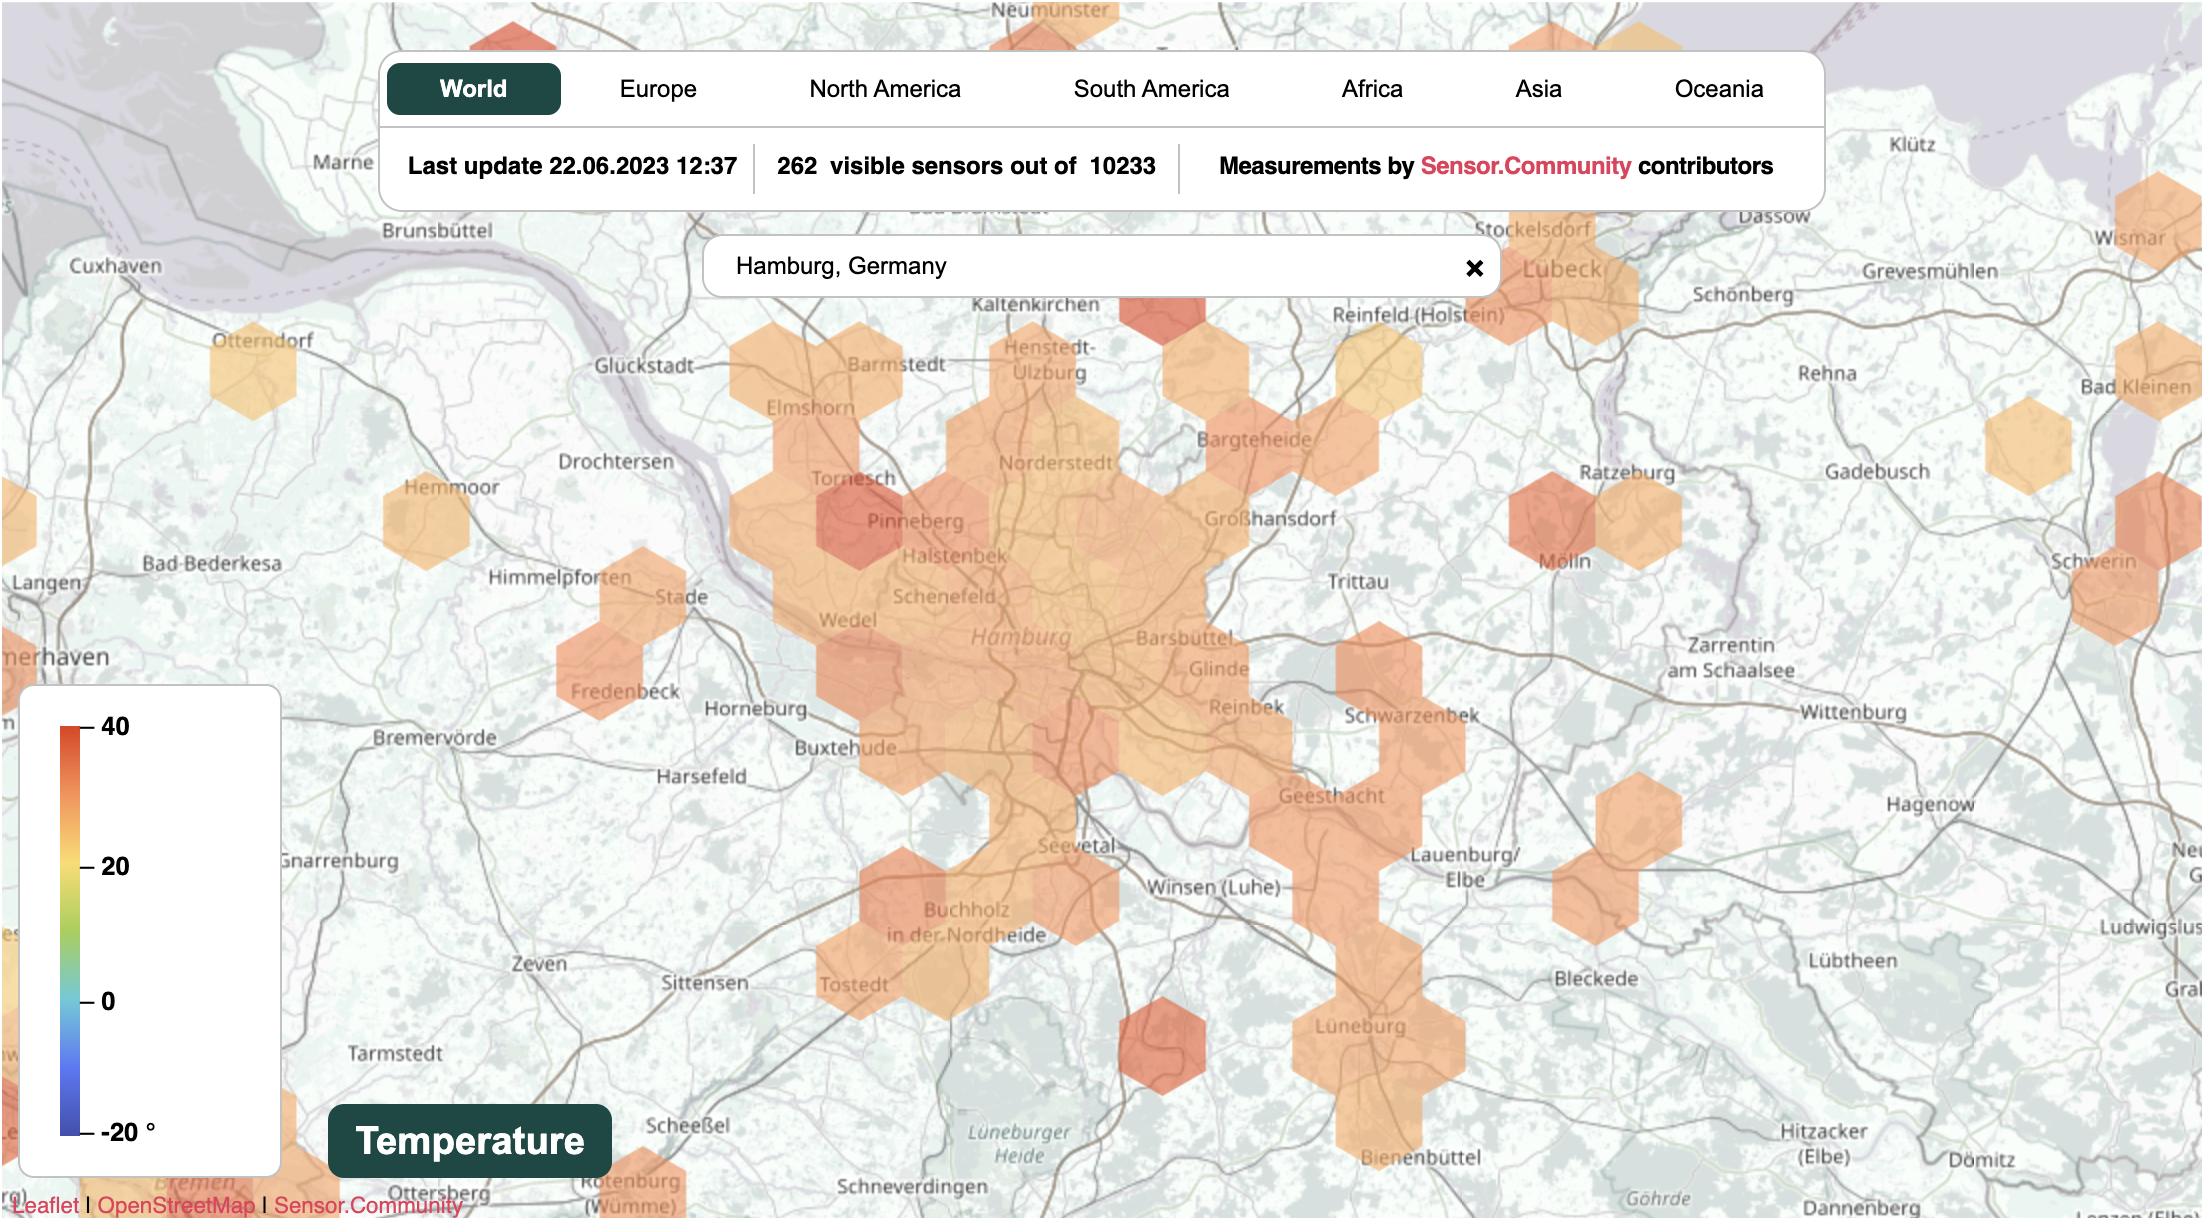
\includegraphics[width=0.8\textwidth]{images/sensor_community_temperature_map.png}
    \caption{Temperature map from Sensor Community for Hamburg, Germany, on 22.06.2023 12:51h with the DWD reference at 25°C}
    \label{fig:temperature_sensor_community_map}
\end{figure}

\begin{figure}[ht]
    \centering
    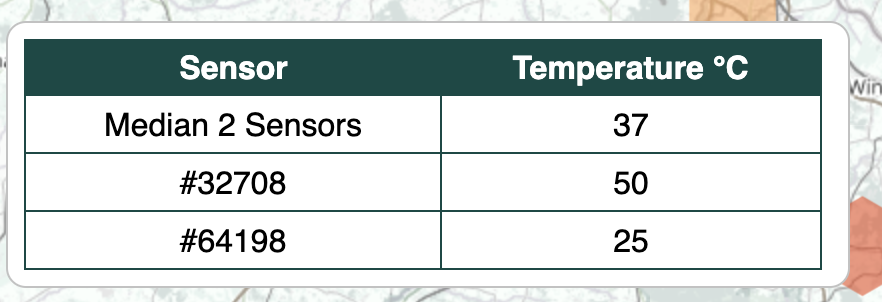
\includegraphics[width=0.8\textwidth]{images/sensor_community_outliers.png}
    \caption{Temperature outlier from Sensor Community for Hamburg, Germany, on 22.06.2023 12:51h with the DWD reference at 25°C}
    \label{fig:temperature_sensor_community_outlier}
\end{figure}

Overall, there are around 11.738 active sensors~\footnote{as of 24.06.2023}. Of these sensors, many are located in Germany and almost half of them are of type BME 280, which is a lost-cost Bosch sensor which can measure temperature, pressure and humidity, as seen in appendix~\ref{sensor_community_sensors_by_countries}.
% Todo: show sensor locations for Hamburg

\subsubsection{Netatmo}



% TODO: add following points
- supervised learning -> target feature, e.g. air temperature\\
- no static sensor locations, e.g. moving sensors -> can be simulated via leaving out data points\\
- spatial and temporal influence between features\\
- data quality -> missing values, outliers, wrong values, ...\\

data from Netatmo, and data from the german weather services (DWD) which serve as reference points,

\section{Overview Data Sources}

With the rise of the Internet and Big Data, the amount of available data has increased exponentially in the last decade. Additionally, movements such as the OpenData movement have made many datasets publicly available and promoted collaboration in research. There are many different data sources available that can be categorized as fully open source, OpenData, or commercial.\\
% Open source data sets -> user generated (e.g. OpenStreetMap)
Open source data sets can be found via... A very popular example is the OpenStreetMap project, which aims to ...\\
% OpenData -> government, research, ...
OpenData...\\
% Commercial -> satellite data, weather data, ...
Example for commercial data providers are Netatmo...\\

Reference data: DWD station data (see https://dwd-geoportal.de/products/OBS\_DEU\_PT10M\_T2M/) -> 10 min 2m height air temperature
https://opendata.dwd.de/climate\_environment/CDC/observations\_germany/climate/10\_minutes/air\_temperature/recent/

need to write script to download all files and for each file do some conversion to csv
% Build Netatmo api connector, load data

- overview of sources for good datasets for temperature and climate related research

goal:
- collect mutiple datasets (many features, fine-granualar spaciotemporal)
- enhance datasets with additonal information (soil conditions, zoning plans, vegetation health)


\section{Feature Engineering}

The goal of feature engineering is to create features from the available data that can be used as input for the machine learning models. The process includes the selection of features, the extraction of features from the raw data, and the transformation of features into a format that can be used by the machine learning models.
The target feature in this work is the air temperature at 2m height. The input features are a combination of sensor readings from weather stations, sensor networks such as Sensor Community and Netatmo, as well as additonal meta data such as soil conditions, zoning plans, vegetation health, and satellite data.\\

- target variable: air temperature
- input features:
    - weather station measurements (air temperature, humidity, wind speed, wind direction, percipitation)
    - satellite data (surface temperature, surface roughness, soil temperature, land coverage indexes, sky view factor, ...)

    Need to separate between reference grade data (weather station calibrated), and low-cost sensors without placement information

% \section{Access to data sets}
% \label{sec: access to data sets}

% % overview of data collection
% % - open data movement
% %     - list open data catalogues (EU, more local ones)
% % - commercial sources
% %     - list some examples, but not focus because not accessible
% % - overview data preperation
% % - overview of feature selection
% % - overview ML interpolation methods

% As part of this thesis, the collection of own data via sensors or other means is not feasible due to time and resource constraints. However, there are many onlie sources and portals/catalogues that give access to a wide variety of data-sets.

% \subsection{OpenData Movement}
%  - portals
%         - official:
%             - EU: https://data.europa.eu/data/datasets?query=temperature\&locale=en (combinas many governmental and local catalogues) / https://data.europa.eu/data/catalogues?locale=en
%             - USA: https://data.gov/
%             - UK: https://www.data.gov.uk/
%         - private: https://www.kaggle.com/

% - strategies:
%     - self procurement (test beds -> Helsinki Testbed (climate research meso sclae), UK Birmingham Testbed (climate + smart city), )
